%%%%%%%%%%%%%%%%%%
% 			 
%			Master Thesis - UWB
%				Introduction code
%
%			Author : Wilson Daubry
%
%%%%%%%%%%%%%%%%%%

\chapter{Introduction}
\pagenumbering{arabic} 
\setcounter{page}{1}
\label{introduction}

Nowadays, indoor localization is a growing feature of many smart buildings, either to allow the navigation of autonomous robots, navigate in an unknown building using a indoor version of the \gls{gps}, etc. The widespread \gls{gps} is not suited for indoor localization \cite{bejuri2013ubiquitous} \cite{kulmer2017using}, in this scope, an indoor locating system using the \gls{uwb} technology and based on trilateration has been developed in \cite{hannotier2019indoor}.
\vspace{2mm}

This locating system locates a mobile device, called tag using three fixed beacons, named anchors, placed at known position. The schematic of this system is shown in Fig. \ref{fig:schem_loc}. The tag is mainly composed of an \gls{uwb} antenna and a smartphone with a custom android application developed to display the position and orientation of the tag on a given map.

\begin{figure}[H]
\centering
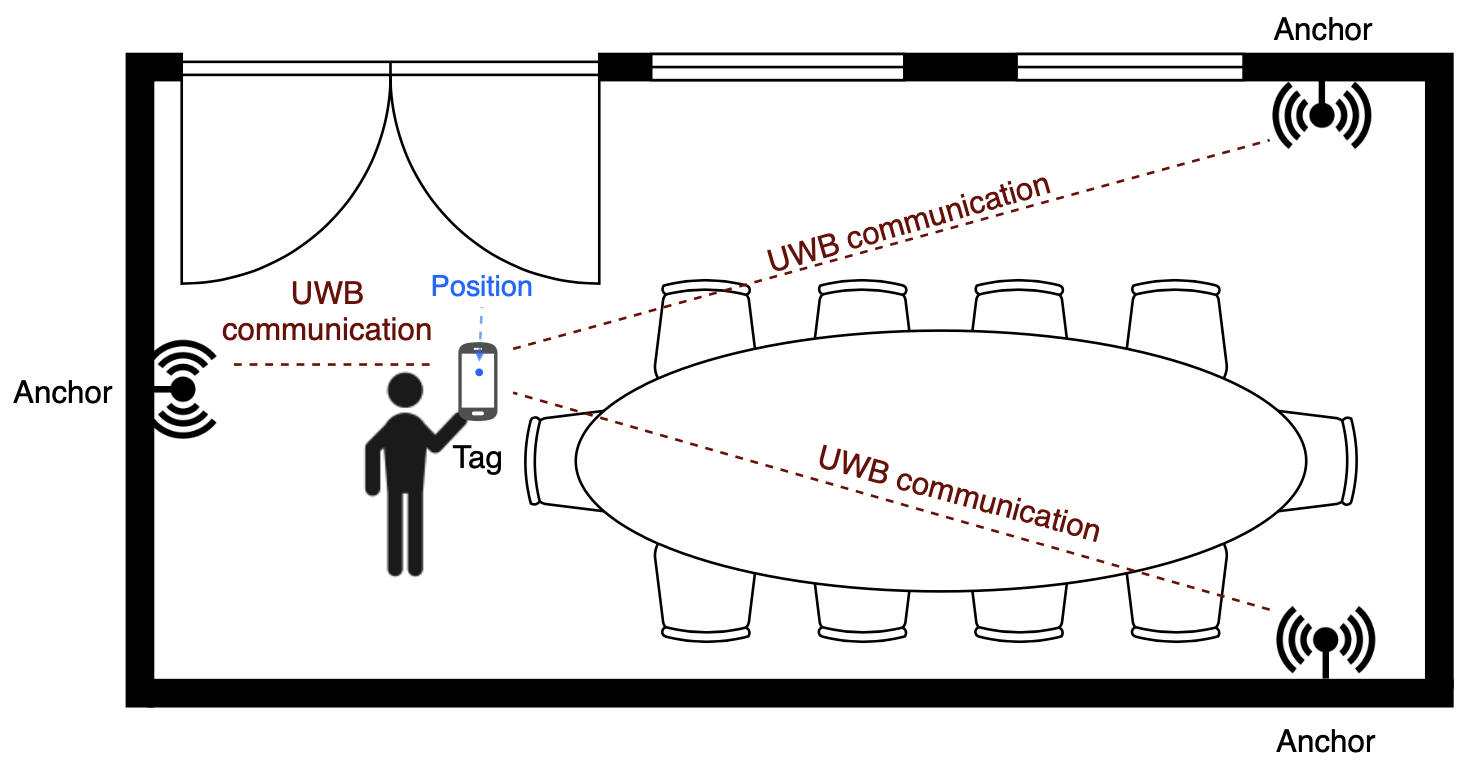
\includegraphics[width=.8\linewidth]{Images/schem_loc.png}
\caption{Schematic of an indoor locating system, a tag interacting with three anchor to know its position in the room. Taken from \cite{hannotier2019indoor}.\label{fig:schem_loc}}
\end{figure}

This locating system is based on the assumption that a \gls{los} between the tag and the anchor is always clear, no object or body obstructing it. Since this can not be guaranteed for every location at every moment for indoor location, two main possibilities occurs. The first one is to increase the number of available anchors, statistically increasing the probability to always have two \gls{los}. This approach has been studied in \cite{guyard2019navigation}. The second approach, is to develop a locating system that may function with less than three antennas available. This thesis focuses on this second approach, studying and qualifying a locating system using only one anchor.
\vspace{2mm}

In the second chapter, a state of the art is presented, summarizing the previous work made on \gls{uwb}, \gls{rtls}, indoor locating systems, describing the functioning of the locating system implemented in \cite{hannotier2019indoor} and detailing the theory behind the some one anchor  locating systems. In the third chapter, two different algorithms developed to perform the indoor localization using only one anchor are presented.
\vspace{2mm}

Chapter four focuses on the simulation developed to test and study the algorithms developed in chapter \ref{algos}. The functioning of the simulation is first presented and the simulation results of the two algorithms are then presented. The fifth chapter focuses on the implementation and modification of the experimental set-up in order to test and extract experimental data to test the algorithms in a real environment.
\vspace{2mm}

The last chapter comes back on the work carried out and the results obtained during this thesis, outlining the research avenues that should be investigated in further work, concluding this thesis.
\vspace{2mm}

\subsubsection{Message to the reader}

Before reading this thesis, the reader must be warned that the last section will seems rather unfinished. Due to the COVID-19 situation and the resulting lock-down, the experiment part, which was supposed to be the main focus of this thesis, was compromised. From that moment, the scope of the thesis was reoriented towards simulations that should be as realistic as possible in order to conduct the same sort of analysis as would have been done using experimental data.